\RequirePackage{filecontents}
\begin{filecontents}{refs.bib}

@online{haar,
title = {Tutorial On Haar Cascades},
url = {http://docs.opencv.org/trunk/doc/py\_tutorials/py\_objdetect/py\_face\_detection/py\_face\_detection.html},
organization = {OpenCV},
year = {2014},
urldate = {2015-01-06},
}

@online{git,
ALTauthor = {Joe Howse},
ALTeditor = {editor},
title = {haarcascades},
url = {https://github.com/Itseez/opencv/tree/master/data/haarcascades},
organization = {OpenCV},
day = {27},
month = {dec},
year = {2014},
urldate = {2015-01-06},
}

@INPROCEEDINGS{990517,
author={Viola, P. and Jones, M.},
booktitle={Computer Vision and Pattern Recognition, 2001. CVPR 2001. Proceedings of the 2001 IEEE Computer Society Conference on},
title={Rapid object detection using a boosted cascade of simple features},
year={2001},
month={},
volume={1},
pages={I-511-I-518 vol.1},
doi={10.1109/CVPR.2001.990517},
ISSN={1063-6919},}

@online{marco,
author = {Marco Becerra},
title = {Leg Detector},
url = {https://github.com/marcobecerrap/leg\_detector},
day = {12},
month = {nov},
year = {2014},
urldate = {2015-01-06},
}

@ARTICLE{4695975,
author={Bellotto, N. and Huosheng Hu},
journal={Systems, Man, and Cybernetics, Part B: Cybernetics, IEEE Transactions on},
title={Multisensor-Based Human Detection and Tracking for Mobile Service Robots},
year={2009},
month={Feb},
volume={39},
number={1},
pages={167-181},
doi={10.1109/TSMCB.2008.2004050},
ISSN={1083-4419},}

@online{ros,
title = {ROS.org},
url = {http://www.ros.org/}, %core-components/},
organization = {Open Source Robotics Foundation},
urldate = {2015-01-06},
}

@online{rospy,
title = {rospy - ROS Wiki},
url = {http://wiki.ros.org/rospy},
organization = {Open Source Robotics Foundation},
day = {31},
month = {dec},
year = {2013},
urldate = {2015-01-06},
}

@ARTICLE{75902,
author={Cox, Ingemar J.},
journal={Robotics and Automation, IEEE Transactions on},
title={Blanche-an experiment in guidance and navigation of an autonomous robot vehicle},
year={1991},
month={Apr},
volume={7},
number={2},
pages={193-204},
doi={10.1109/70.75902},
ISSN={1042-296X},}

@book{Murphy:2000:IAR:517685,
 author = {Murphy, Robin R.},
 title = {Introduction to AI Robotics},
 year = {2000},
 isbn = {0262133830},
 edition = {1st},
 publisher = {MIT Press},
 address = {Cambridge, MA, USA},
}

@online{pp,
author = {Peter Parente},
title = {pyttsx - Text-to-speech x-platform},
date = {2014-08-24},
url = {http://pyttsx.readthedocs.org/en/latest/},
urldate = {2015-01-13},
}

@inproceedings{Fikes:1971:SNA:1622876.1622939,
 author = {Fikes, Richard E. and Nilsson, Nils J.},
 title = {STRIPS: A New Approach to the Application of Theorem Proving to Problem Solving},
 booktitle = {Proceedings of the 2Nd International Joint Conference on Artificial Intelligence},
 series = {IJCAI'71},
 year = {1971},
 location = {London, England},
 pages = {608--620},
 numpages = {13},
 url = {http://dl.acm.org/citation.cfm?id=1622876.1622939},
 acmid = {1622939},
 publisher = {Morgan Kaufmann Publishers Inc.},
 address = {San Francisco, CA, USA},
} 

@book{Thrun:2005:PR:1121596,
 author = {Thrun, Sebastian and Burgard, Wolfram and Fox, Dieter},
 title = {Probabilistic Robotics (Intelligent Robotics and Autonomous Agents)},
 year = {2005},
 isbn = {0262201623},
 publisher = {The MIT Press},
} 

@online{kl,
title = {Probabilistic Roadmap Method (PRM)},
url = {http://www.kavrakilab.org/robotics/prm.html},
organization = {Kavraki Lab, Rice University},
urldate = {2015-01-13},
}

@online{stan,
title = {Motion Planning in Robotics},
url = {http://cs.stanford.edu/people/eroberts/courses/soco/projects/1998-99/robotics/basicmotion.html},
organization = {Stanford University},
urldate = {2015-01-13},
}


\end{filecontents}

\documentclass[10pt]{article}
\usepackage{times}
\usepackage[backend=biber,style=authoryear]{biblatex}
\usepackage[british]{babel}
\usepackage{courier}
\usepackage{listings}
\usepackage{array}
\usepackage{graphicx}
\usepackage{gensymb}
\usepackage[margin=1.1in]{geometry}
\usepackage{fixltx2e}
%\usepackage{hyperref}

\addbibresource{refs.bib}

\begin{document}

\title{Intelligent Robotics --- Call A Meeting}

\author{Jack Browne, Jack Jacques, Hugh Samson, and Matthew Williamson}
\date{\today}
\maketitle

\section{Introduction}

This report aims to present a solution to the ‘Call A Meeting’ task. The objective of the task was for the Pioneer 3-DX robot to autonomously locate an empty room suitable for holding a meeting and then find two people in the lower ground floor of the University of Birmingham Computer Science Building and bring them to the meeting. The robot had 15 minutes to complete this task and was penalised whenever a human had to intervene to correct its behaviour. The solution we will present consisted of several different algorithms and techniques, the background of these are presented first in this report. This is then followed by more specific descriptions on how these techniques were applied in conjunction with one another and the design elements involved to create the overall solution. There is then data on the experiments that were performed to help determine which methods to use and how to refine them. Finally, we attempt to evaluate our solution  and discuss its performance alongside possible improvements.

\section{Background}

\subsection{Control Architecture}

For a robot to be autonomous it must be able to decide on an appropriate action to take using its internal sensors, external sensors and knowledge of the problem at hand. This section of the report will detail the two main paradigms for robot control; hierarchical/deliberative and reactive.

\subsubsection{Hierarchical/Deliberative Paradigm}

A robot has three primitive functions:

\begin{itemize}
\item Sense - taking data readings from sensors and translating the readings into useful information
\item Plan - using the information from sensor readings and deciding on a task for the robot to perform
\item Act - carrying out a task, by giving commands to the robot’s motor actuators
\end{itemize}

A robot using a hierarchical paradigm, such as Shakey using the STRIPS planner \parencite{Fikes:1971:SNA:1622876.1622939}, will always carry out these three tasks sequentially; sense, plan, act \parencite{Murphy:2000:IAR:517685} as shown in figure 1. The next action is always explicitly planned out, no matter how trivial the resulting action might be. 

\begin{figure}[h]
\centering
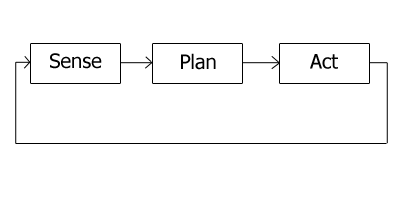
\includegraphics[scale=0.4]{Hierarchical}
\caption{The Hierarchical/Deliberative Paradigm}
\end{figure}

Also, the hierarchical paradigm must maintain a global model of the world which must be updated whenever new data is sensed and is then used by the planner to plan the next action. This causes two issues, firstly it must make a ‘closed world assumption’. Meaning that the global model has all of the information that the robot will ever need to plan it’s next action; in dynamic environments this is often not that case. This can make the global models very difficult to work with.

The second issue is the ‘frame problem’. How do we build and maintain a representation of the world that is \textit{just} detailed enough? If the model is not detailed enough there may be some events that we cannot plan for. However, if the model is too detailed the planning may become intractable.

\subsubsection{Reactive Paradigm}

\begin{figure}[h]
\centering
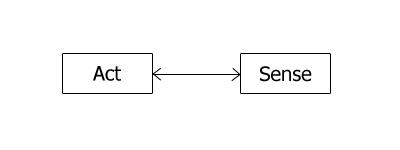
\includegraphics[scale=0.4]{Reactive}
\caption{The Reactive Paradigm}
\end{figure}

In the hierarchical paradigm there is a bottleneck at the planning stage; planning is generally quite difficult. One solution to this problem is to remove the planning stage all together! This is how the reactive paradigm works. It is simply a sense-act pairing, as shown by figure 2.

Using the reactive paradigm the sensors are effectively connected directly to the robot’s actuators and a given sensor reading will cause a specific reaction from the actuator. For example, suppose we have a robot with three range sensors (left, right and middle), we might say that given a reading of less than 0.5m from the middle sensor the robot should stop forward motion. We could then expand this to say that a reading of less than 0.5m from the left sensor causes the robot to turn right. It might be thought that these ‘reactions’ would interfere with each other, however each of these sense-act pairs are running in parallel; causing the robot to stop forward motion and turn on the spot. Each of these pairings should be a fairly simple behaviour. 

There is no internal state or memory in a reactive robot because it does not require a global world model in order to decide on the next action, it simply reacts to the sensor readings. This makes reactive robots generally more efficient and cheaper to build. Their lack of a world model also means they can often perform better in dynamic environments, since they make no assumptions about the world they are in. 

\paragraph{Hybrid Paradigm}

Sometimes, planning is necessary. Not everything can be achieved using purely reflexive actions. This has led the emergence of hybrid paradigms where a planner is used the break the task down and to decide the necessary behaviours. These behaviours would then be executed using a reactive approach

\subsection{Localisation}

Localisation is the task of (reasonably) accurately estimating a robot's position in a world, given a map and a stream of sensor readings. This task is said to be “the most fundamental problem to providing a mobile robot with autonomous capabilities.” \parencite{75902} Even the simplest of tasks, such as moving to a position in the world, would be almost impossible without the robot knowing its current position.

The basic approach to localising a mobile robot is to use some sort of range finder and then compare the readings of this to the expected distance of the walls/obstacles as given by the map. From this we can determine the most likely position of the robot. 

Sensor information is undoubtedly noisy and the map is inherently inaccurate due to the dynamic environment in which we are operating. This means we cannot accurately reason about this robot’s location without taking this uncertainty into account. We do this using recursive probabilistic techniques, which attempt to quantify the uncertainty.
\subsubsection{Bayes Filter}

The general aim of all of these recursive probabilistic techniques is to maintain and update an ongoing belief about the state of the robot, $X$. This belief is represented in form of a probability distribution. The belief at time $t$ is represented by $x_t$. To update this belief we must use some sensor data, $z_t$, and our control data (actions), $u_t$. From this we can build the following:

\begin{itemize}
\item A sensor model $P(z_t|x_t)$ - the likelihood of seeing a giving sensor reading, given the current state.
\item An action model $P(x_t|u_t,x\textsubscript{t-1})$ - the likelihood of a particular state, given the state we were previously in and the action taken
\end{itemize}
 
We can then say that our belief $Bel(x_t) = P(x_t| z\textsubscript{1:t}, u\textsubscript{1:t})$. In other words, the likelihood of being in a given state at time $t$ given all of the previous control data and sensor data. A major problem with this is the unbounded size of $t$, which could make these problems intractable. However we are able to bound this by making a Markov Assumption which says that the current state only relies on the state that immediately preceded it.

The filtering then happens in two steps. Firstly the prediction, where we predict how the new state should look based only on the control data. Then the update, where the predicted state is updating using the new information we have - the sensor data. The update happens according the Bayes’ rule. This is then applied recursively every time new data in received, the new state becomes $x\textsubscript{t-1}$ in the next iteration of the algorithm.

\subsubsection{Kalman Filter}

The Kalman filter is an implementation of the Bayes’ filter, that makes some assumptions about the world in order to make the algorithm tractable:
\begin{itemize}
\item The action model $P(x_t|u_t,x\textsubscript{t-1})$ is a linear function with gaussian noise
\item The sensor model $P(z_t|x_t)$ is a linear function with gaussian noise
\item The initial belief, is normally distributed
\end{itemize}

There are many world models will not fit these assumptions, however there are also many that will which is why the Kalman filter is still widely used even though it is about 60 years old. \parencite{Thrun:2005:PR:1121596} 

The Kalman filter, being a gaussian filter, will always return a gaussian distribution. This makes Kalman very efficient, one of the primary reasons that it is still in use today. It does have some drawbacks, particularly when it comes to localisation problems. The assumption of linearity being the most prevalent since often this cannot be assumed for robot systems. Also, the gaussian restriction means that a Kalman filter cannot keep track of multiple hypotheses, this makes it very difficult to recover from a failure in localisation.

\subsubsection{Particle Filter}

The particle filter is another implementation of the Bayes filter, a nonparametric implementation. This filter does not make any assumptions about the world in the way that the Kalman filter does.

The belief is represented by a set of samples, possible locations of the robot. It may then be decided that the most likely of these samples to be the actual location of the robot is one in the most densely populated cluster of particles, or maybe the average particle location (although this probably isn’t a good solution).

This algorithm works in three steps:

\begin{enumerate}
\item Firstly the particles are all updated based on the control data $u$ to construct a new temporary set of particles
\item The temporary set of particles are all then weighted, using the sensor data $z$. If the sensor data correlates with the expected data for a given particle, this particle will have a high weight, and vice versa. 
\item The actual filtering happens by a process of importance resampling. A completely new set of particles are generated based on the weights from the temporary set. A highly weighted particle should have more chance of being ‘chosen’ than a lowly weight particle. 
\end{enumerate}

The result of this should be a new set of particles which have all shifted towards highly weighted/more likely particles from the previous set. A “survival of the fittest” approach.

The particle filter is used for localisation in an algorithm called Monte Carlo Localisation. A potential problem with this is particle deprivation. This occurs because in order for a particle to even be considered in the sampling it must be in the original set. If all of the particles converge on an erroneous location it will become impossible for the particle filter to recover. This can be avoided by implementing an augmented version of the Monte Carlo Localisation algorithm; in this augmented version particles are added randomly around the sample space. The number of random particles should be proportional to how accurate you believe the localisation is.

Another problem with the basic Monte Carlo Localisation algorithm, and particle filter in general, is that it can be very inefficient. This is because a large number of particles, likely over 1000, are needed to accurately localise in the first place. The algorithm has linear complexity, with respect to the number of particles.  1000 is fine if the robot is actively localising because it does not know where it is, however if the robot is well localised and is simply maintaining a prediction 1000 particles is excessive! A way to improve this efficiency is by adapting the number of particles based on how confident you are in the estimate. This is known as Adaptive Monte Carlo Localisation.

\subsection{Navigation and Movement}

It was soon realised that there would need to be two different `types' of movement code, one to localise the robot when it's first initialised, and another to guide the robot using path planning while still avoiding collisions, after localisation.

To do this we looked at both the Navigation Stack within rospy, and our own implementations of movement. The former had the added benefit of being simple to use within a SMACH state machine, as it's set up as an action server. The Navigation Stack also employs local and global costmaps, which means that the robot can avoid collisions, and replan if it needs to find a completely new path. There are numerous ways to guide a robot through its configuration space, two such approaches are outlined below.

\subsubsection{Probabilistic Roadmap}

A probabilistic roadmap approach has two stages; the learning phase, and the query phase. In the learning phase a large number of random points are generated in the configuration space C\textsubscript{free}, from there the robot tries to create edges between these points - either between each of the point's K Nearest Neighbours, or within a certain diameter of the point - ensuring to stay within C\textsubscript{free} i.e. not create a route that is obstructed. In the query phase the start and goal graph is traversed to find the quickest path using an algorithm such as A* search or Djikstra's Algorithm. Depending to the positioning of the initial distribution of particles and the amount of random particles the Probabilistic Roadmap may not always return a result if there is one, and so the number of particles has to be enough so that it finds a path, but not so many that the system becomes totally inefficient.

\subsubsection{Cell Decomposition}

Cell Decomposition involves splitting the configuration space into smaller regions, or cells. \parencite{kl}
After doing so adjacent regions are then used in a connectivity graph which is used to find a path by following adjacent free cells from the start to goal. Cell decomposition can be done either in an ‘exact’ or ‘approximate’ approach. Exact Cell Decomposition is complete and will always find a path, if there is one, but is a more complicated algorithm. Approximate Cell Decomposition often comes up with the same results as its partner, and is easier to program, but is not always complete. \parencite{stan}
%Probablistic Roadmaps || Other path planning algorithms (Cell Based)
%Any grid search

\subsection{Person Detection}

Detecting the presence of a human was a critical part of the task and something in which multiple potential methods had to be researched and compared. The robot needed to be able to detect a person with enough confidence to ask them to come to the meeting and then repeat this with another person. Here we will talk about different approaches to detecting people; one which uses the robot’s camera and two that use the laser range scanner.

\subsubsection{Haar-Cascade}

One possible approach is to use a mounted camera in order to detect the faces of people in the vicinity. This can be achieved through the use of Haar-cascades \parencite{haar}. Which are based upon the principles described in the paper ‘Rapid Object Detection using a Boosted Cascade of Simple Features’ \parencite{990517}. 

The Haar-cascades work by converting an image into greyscale, and applying a cascade of classifiers to help judge it as a face or not. This results in an incredibly efficient, machine-learning based, face detection system. The system uses Adaboost which has trained a set of classifiers by looking at the features of thousands of images of faces and images without faces. To optimise the speed of this process, the system applies the best classifiers (that is, the features which are the most definitive in what is a face and what isn’t) first and discards the results that return negative. Then on the remaining positive results, applies the second classifier to further filter the results. This happens for a large amount of classifiers, removing the need to apply classifiers many times to lots of features. 

The result is a fast and accurate face detection algorithm. Using a different set of classifiers this could easily be adapted to detect other parts of the human body.

\subsubsection{Laser Range Scanner}

An alternative method of detecting people is to use the laser range scanner of the robot. This is ideally placed to detect the legs of a nearby person.

One possible way of using the laser range scanner is a purely machine learning based approach. Given a large enough training set it would be possible to set up a supervised learning experiment to accurately detect the legs of people. The results of this could then be further improved by using a boosting algorithm such as AdaBoost. In order to get accurate results a very large training set would be required - containing differently sized legs in different orientations.

Another way is to use the ideas presented by Hu and Bellotto. They describe an efficient way of detecting legs which is based more on pattern recognition and edge detection \parencite{4695975}. The paper recognises 3 distinct leg positions which can be identified by the laser scanner; ‘two legs apart (LA), forward straddle (FS), and two legs together or SL. The first pattern is usually very common in case the person is standing in front of the robot. The second, however, is most likely to happen when the person is walking. The last pattern covers most of the remaining postures; often, however, it can also be generated by other objects in the environment.’ The readings are processed into an array of string readings. The readings are then pattern matched against the 3 leg positions described above to determine whether it is a leg. The distance and location of the leg is also calculated by the midpoint of it’s regular expression pattern. The location of the legs were necessary for experimentation but not needed in the solution.

\section{Design and Task Approach}

\subsection{System}

\subsubsection{Hardware}

The hardware of the system comprised of a Pioneer 3-DX, a robot with two wheels and a caster and two motors which, accompanied with a differential drive system, give it the ability to turn on the spot. The unit is 455mm wide and 381mm long - it is also 237mm high, without the addition of a tripod and Logitech webcam that was attached for the solution. It also has a Hokuyo Laser Scanner mounted on the front which has the ability to detect objects clearly up to 4m away in a range of 240 degrees.

Attached to the computer is a Toshiba Dual-Core i3 laptop running a Ubuntu 12 operating system. This operating system can then run the necessary components of the ROS (robot operating system) supplied.

\subsubsection{Software}

The Pioneer uses ROS - Robot Operating System. It has very low-level controls over all the hardware of the robot and its peripherals and at it’s very core it can be used to easily pass messages between topics. The details of this inter-communication between nodes of control is managed by an ‘anonymous publish/subscribe mechanism.’

ROS allows many languages to be used to when developing code. Python was the language used for the solution mainly because of the rospy \parencite{rospy} library which allowed development to be tested immediately on the robot immediately after making changes. Python is a scripting language so optimisation of code was important in run-time performance but the API and it’s interface with ROS Topics, Servers and Parameters saved much time throughout development which would not have been achieved with another programming language.

\subsection{Detailed Procedures}

\subsubsection{Control Architecture}

As with most ‘paradigms’ the eventual solution fell somewhere in the middle of the two extremes. We felt that the environment was too unstructured for us to be able to build an effective global model. This ruled out using a purely hierarchical paradigm. However, our robot would require some ability to plan it actions ahead of time. This ruled out using a purely reactive paradigm.

We had identified early on that the task could well represented as a finite state machine; due to the clear breakdown of tasks and the natural progression between tasks at all stages. We developed the following state machine to help guide us through our solution to the task.

\begin{figure}
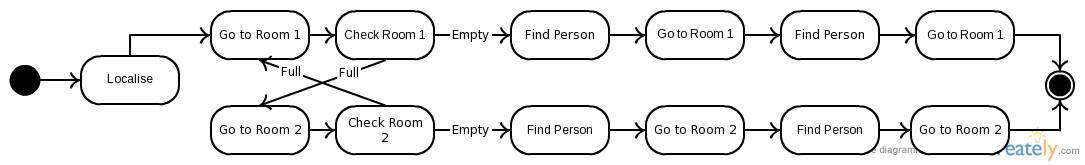
\includegraphics[width=\textwidth]{ca}
\caption{Our Finite State Machine}
\end{figure}

\paragraph{SMACH}

Looking at the ROS libraries we found a state machine library called SMACH, this library had many features which made it desirable for our purposes.  It had the ability to use ROS’s Action Server libraries, this meant we could implement all of our behaviours as a ROS action, as well as use the preinstalled ROS actions, and then easily incorporate them into the overall architecture. Also, a feature that became apparent after we began experimenting with ROS was that it easily allowed us to implement a hierarchical state machine. This would be important because our final state machine would be much larger than the original design.

\paragraph{Final State Machine}

Through the use of a hierarchical state machine we were able to simplify the overall state machine to just four logical states:

\begin{itemize}
\item Localise
\item Find empty room
\item Fill room 1
\item Fill room 2
\end{itemize}

‘Find empty room’ handles the moving between the two rooms and checking whether they are empty, using four states of its own. When an empty room is found either ‘1’ or ‘2’ is returned, depending on which room was found to be empty. The state machine for checking whether a room is empty contains six states. 

‘Fill room 1’ and ‘Fill room 2’ handles finding two different people and bringing them to the empty meeting room. Each of these state machines contains four separate states. Two of which are themselves state machines containing three states.

It is clear that we have been able to use the hierarchical state machine to our advantage to modularise the control of the robot. This allowed us to simplify the overall state machine making it easier to understand and maintain. While at the same time continually adding the layers of complexity necessary to complete the task. The modularisation also helped hugely in the testing of our code and experimentation, as we could easily execute one specific behaviour in isolation.

\subsubsection{Localisation}

We decided that the most appropriate approach to localisation for this task would be Monte-Carlo Localisation implemented with a particle filter and utilising the Markov assumption.

We had previously developed an implementation of the Augmented MCL algorithm as described by \cite{Thrun:2005:PR:1121596}. However after testing it became clear that this implementation would localise well enough for this task. Also we had not managed to implement the adaptive side to the algorithm, which means that the computation would become inefficient when using the large number of particles needed to localise initially.

We decided instead to use the AMCL package included with ROS, the middleware that we were already using. This had the added advantage of tying in with the other behaviours that we had already implemented.

\subsubsection{Navigation and Movement}

Two different approaches for navigation and movement were used, the Navigation Stack - as seen in figure 4 - and our own random movement code. When localising the robot at the beginning of a run the latter was chosen, as Navigation Stack relies on the implementation of AMCL in rospy and therefore the robot needs to be localised \textit{before} it can be used. The code told the robot to turn whenever it found a wall, and when it `localised' (defined as when the pose array for AMCL dipped under 1000 poses) it then switched to using Navigation Stack instead.

On localisation the robot would build a path to the first meeting room -- where it would check if it was empty -- if not then it go to the other meeting room and check there. As described in 3.2.4, for the purpose of people detection points were set up that would allow the robot to check for humans in every part of the space, the robot then moved between these points. It did its own path planning within Navigation Stack using a probabilistic road map and stopped collisions by using a local costmap. We ran tests to discover whether the costmap was the right size or not in 4.1. When a person was found the robot would then build a path back to the empty meeting room in order to take them there. The Navigation Stack was also more acceptable because it was directly compatible with SMACH; by passing a goal to move\_base the robot would plan its path, move to the goal, and all while avoiding collisions.

\begin{figure}
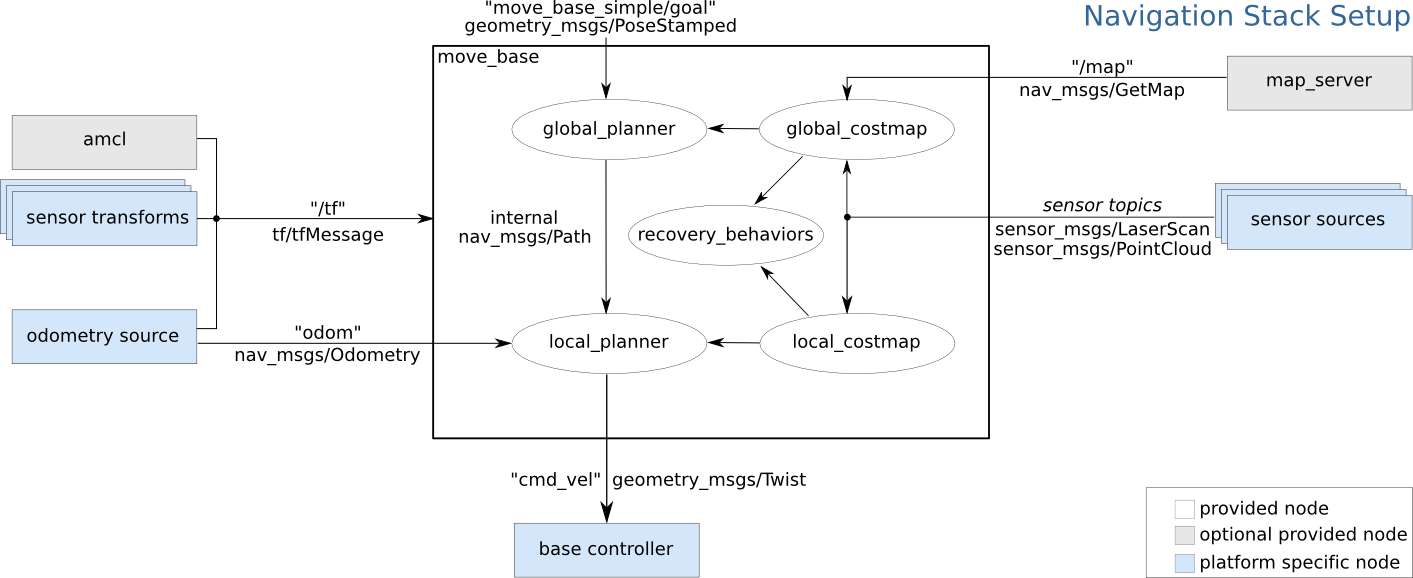
\includegraphics[width=\textwidth]{ns}
\caption{The Navigation Stack}
\end{figure}


We chose to use a Probabilistic Road Map as both PRMs and Cell Decomposition approaches aim to solve similar problems and therefore also have similar faults, however we have more control over the PRM as the values - such as costmap inflation - are easier to modify than the CD algorithm. Especially as PRM was already implemented within the ROS Navigation Stack which made it much more appealing than its counterpart.

\subsubsection{Person Detection}

We split the person detection into two distinct parts. Detecting people in a room and detecting potential conferees for the meeting. This was because although essentially the same task, they had different considerations. When detecting people in a room it was important that we did not get any false negatives, declaring the room to be empty when it was actually full. When looking for conferees the primary concern was reducing the number of false positives in order to reduce the complexity.

\paragraph{Checking a Room}

For this we used the principles described in 2.4.2 and code adapted from Marco Becerra, who demonstrates for the module, available on Github \parencite{marco}.

Experimentation showed the results of this were very varied; but allowed us to approximate the best parameters for detecting legs. Yet, false positives were still generated in the ROC analysis. Although our primary concern was to avoid false negatives it was still important that we dealt with them. Looking at a visualisation of the laser scans we noticed that the false positives were consistently appearing in the same location, this enabled us to come up with a solution by simply taking these false positives into account. We also observed that the false positives had a tendency to flicker between scans, particularly as the robot moves. Whereas a true positive would be much more stable. This helped our solution because it meant that if a person was standing in an area where there is ordinarily a false positive it should still report that the room is full.

To do this we needed to obtain a base value for each room. This was done by rotating the robot on the spot while scanning the room for legs. The robot then summed the number of readings in which legs were detected and divided it by the total number of readings to get an average. Testing was performed a number of times for this and an average and minimum were found for rooms being empty and full. For certainty, the minimum number was used of the ‘non-empty’ room  - if readings were below this threshold then the room was deemed ‘empty’. Because of the occasional anomaly, it was decided that the procedure be performed twice and only if both times the room is seen as ‘empty’ will the robot continue. These modifications vastly improved reliability.

\paragraph{Finding Conferees}

Experimentation showed that though face detection was extremely accurate, it was unreliable unless the subject was directly facing the camera and not looking from an angle - something which wasn’t guaranteed in a dynamic environment. 

A compromise was found after experimentation with an upper-body-detection Haar-cascade using open-source code obtained from OpenCV’s GitHub \parencite{git}, which used the exact same principle as the face detection but used training data that analysed features of a human upper body. This worked very well in almost all situations except when there was a lack of contrast between the person’s clothing and the background behind them - this made it difficult for the body to stand out in the grey-scale image that was created. In most cases however, the detection was reliable and gave very few false positives in the ROC analysis making it ideal for this part of the task.

The image was taken from a Logitech RGB Webcam, which was mounted on a tripod on top of the device. The webcam was constantly running at a frame rate high enough to capture people but low enough so that it would still be able to run on the laptop without consuming all the CPU. Experimentation showed us that the perfect distance to detect humans was around 2 metres away from the camera. 

Thus, rather than wasting time and CPU power to randomly move around looking for people, we used this information to hardcode coordinate points into our state machine. Once each point was reached the robot would spin 360 degrees to check if a person was in the area. This ensured that a person standing in any part of the room was going to be picked up by the camera. 

Once a person was recognised, we used a simple text-to-speech interface to communicate with the person, requesting the person enter a simple ‘y’ or ‘n’ on the terminal screen if they wanted to come or not come to the meeting respectively. It was realised that a timeout would be needed to ensure that if a false positive was picked up by the body detection, or the person walked away then the robot could continue. 

The text-to-speech interface that was used is called pyttsx \parencite{pp}. It is a simple python library that allows for a request to be made at any time to execute a speech command. This allowed for an ergonomic method for humans to interact with the robot with minimal effort. 

\section{Empirical Study}

\subsection{Costmap Inflation}

\paragraph{Aim}

It was noticed that the local costmap was failing to detect obstacles and driving into them. One of the reasons this can happen is if the robot failed to fully localise before moving onto it’s next state in the state machine. After this was corrected, it was important to test if the costmap could re-plan when the robots goal was blocked.

\paragraph{Method}

The robot was allowed to localise and then its goal was blocked by various obstacles.

\paragraph{Results}

\begin{center}
\begin{tabular}{ |p{2cm}|>{\centering\arraybackslash}p{0.6cm}|>{\centering\arraybackslash}p{0.75cm}|p{6cm}| } 
 \hline
 Object & Find Goal & Time Spent (mins) & Observations \\
 \hline
 $1m ^ 2$ of black paper & Yes & 2 & Built a new local costmap to replan.\\[0.3cm]
 Tall Chair & Yes & 0 & Maneuvered around immediately.\\[0.3cm]
 1.2m board & Yes & 3 & Planned around object, after negotiating past a nearby bin.\\[0.3cm]
 Two chairs with 3ft gap & Yes & 8 & Could not replan through chair gap due to costmap inflation, but could when gap was slightly increased\\
 
 \hline
\end{tabular}
\end{center}

\paragraph{Conclusion}

The results of the experiment allowed us to more precisely plan the robots entry points into the room and reduce the chances of it getting stuck. It also showed that the robot could be trusted to replan if obstacles got in its way.

\subsection{Leg Detection ROC Analysis}

\paragraph{Aim}

To conduct a ROC analysis of the leg detection code to see how reliable it was initially:

\paragraph{Method}

Place robot in multiple environments until 30 legs were detected.

\paragraph{Results}

\begin{center}
\begin{tabular}{ |c|c|c| } 
 \hline
 & Positive & Negative \\
 \hline
 True & 14 & 2 \\
 False & 13 & 1 \\
 \hline
\end{tabular}
\end{center}

Sensitivity: 0.93. Specificity: 0.13

\paragraph{Conclusion}

Leg detection is ‘noisy’, though it was very successful in seeing legs when they were present, it also failed once to see legs, and often detected other objects as legs.

\subsection{Body and Face Detection ROC Analysis}

\paragraph{Aim}

To assess the reliability of both body and face detection techniques.

\paragraph{Method}

Place robot in multiple environments until 30 bodies and 30 faces were detected.

\paragraph{Results}

\begin{center}
\begin{tabular}{ |c|c|c| } 
 \hline
 \textbf{\textit{Face}} & Positive & Negative \\
 \hline
 True & 7 & 12 \\
 False & 3 & 8 \\
 \hline
\end{tabular}
\end{center}

Sensitivity: 0.46. Specificity: 0.8

\begin{center}
\begin{tabular}{ |c|c|c| } 
 \hline
 \textbf{\textit{Body}} & Positive & Negative \\
 \hline
 True & 11 & 8 \\
 False & 6 & 4 \\
 \hline
\end{tabular}
\end{center}

Sensitivity: 0.73. Specificity: 0.53

\paragraph{Conclusion}

Despite the lower specificity, body detection is superior for the needs of the solution due to its increased sensitivity, which is more important.

\subsection{Meeting Room Detection}

\paragraph{Aim}

Find proportion of erroneous leg readings in an empty room compared to readings from a room with legs in.

\paragraph{Method}

This experiment was crucial for deciding when a room was empty or not. The robot was placed in the room at a point that was hard-coded into the map and then made to rotate 360 degrees when legs were and were not present.

\paragraph{Meeting Room A}
\subparagraph{Without People}
\begin{center}
\begin{tabular}{|c|c|}
\hline
 & Average no. people detected over a 360\degree rotation\\
\hline
minimum & 0.0 \\
maximum & 0.075427913682 \\
%3 & 0.037846839285\\
%4 & 0.0\\
%5 & 0.0\\
\hline
\textbf{Average} & \textbf{0.02265495059}\\
\hline
\end{tabular}
\end{center}

\subparagraph{With People}
\begin{center}
\begin{tabular}{|c|c|}
\hline
 & Average no. people detected over a 360\degree rotation\\
\hline
%1 & 0.40173820590 \\
%2 & 0.44843052318 \\
maximum & 0.62987982349 \\
minumum & 0.27124502334\\
%5 & 0.39034824123\\
\hline
\textbf{Average} & \textbf{0.42832836342}\\
\hline
\end{tabular}
\end{center}

\paragraph{Meeting Room B}
\subparagraph{Without People}
\begin{center}
\begin{tabular}{|c|c|}
\hline
 & Average no. people detected over a 360\degree rotation\\
\hline
minimum & 0.351550251245 \\
maximum & 0.58761203289 \\
\hline
\textbf{Average} & \textbf{0.47605412006}\\
\hline
\end{tabular}
\end{center}

\subparagraph{With People}
\begin{center}
\begin{tabular}{|c|c|}
\hline
 & Average no. people detected over a 360\degree rotation\\
\hline
maximum & 1.24989628792 \\
minimum & 0.762219905853 \\
\hline
\textbf{Average} & \textbf{1.08544793725}\\
\hline
\end{tabular}
\end{center}

\paragraph{Conclusion}

The minimum values were used to determine whether a person was present.

\subsection{Optimum Body Detection Distance}

\paragraph{Aim}

To find the optimum distance for body detection to find a person.

\paragraph{Method}

Use the webcam and laptop to see if a box can be drawn in real time around a person. This was repeated multiple times and different distances, with the person standing in multiple angles from the webcam.

\begin{center}
\begin{tabular}{|c|c|c|c|c|c|c|}
\hline
 & Angle & 0 & 45 & 90 & 135 & 180 \\
\hline
Distance & & & & & & \\
1 & & yes & yes & yes & no & yes \\ %Flickers 
1.5 & & yes & no & no & yes & yes \\
2 & & yes & yes & yes & yes & yes \\ %Stable
3 & & yes & yes & yes & yes & yes \\ %Flickers
\hline
\end{tabular}
\end{center}

\paragraph{Conclusion}

We found the optimum distance to be 2m for the body detection to accurately pick up a person standing in multiple poses, this helped us determine the locations of the points on the map to perform body detection.

\section{Discussion}

\subsection{Commentary}

The solution worked well once all the components were brought together. We tested the overall system in different scenarios by measuring the completion time. When being tested in a very busy environment and ensuring the robot had to check both rooms, the overall duration was just below the 15 minute mark - 14:37. This showed that this system should be quick enough to complete the task in all scenarios. In a quiet environment where the robot did not have to stop and replan it completed as quickly as 7:41.

Using the ROS libraries for AMCL and navigation helped with the creating of the system. The advantages of using this were that due to being open source and regularly maintained, these libraries worked well, being more efficient and reliable than what we could have produced in the time given. Although a problem of using this was the functionality could not be easily adapted if necessary.

A particularly successful part of this task was designing our own method for detecting people in a room using the leg detection code. We came up with a novel solution which worked reliably and contributed to our successful overall solution. A potential problem with this is that it is not as general as it could be, since it needs to be calibrated for each room.

\subsection{Improvements}

When running the system we found that the robot-human interaction was not very good. Although the robot will locate and ask one particular person whether they would like to attend the meeting, this is not clear to the human. This is because the robot does not approach or turn to face the person after locating them. This is more of a problem if there is a cluster of people in one small area. It was also not immediately obvious to the person that they needed to press a key in order to respond. An improvement would have been to include speech recognition making for a more natural interaction. 

Another possible improvement might have been to use a Kinect Sensor for human detection. It would have made our human detection a lot more reliable and accurate. With the addition of the depth sensor it would have removed the false negatives from different light levels and the person wearing clothes with similar colours to their background. With the inclusion of the Kinect Sensor we would need a more powerful system to run the solution on as we found from other groups that the Kinect used a lot of processing power to detect people or we could only use the Kinect at certain times to check to definitely make sure someone was there. A potential disadvantage of this would be that the Kinect didn’t work well detecting people while the robot was moving around so this is a compromise we would have to be made.


\printbibliography
\end{document}